% +--------------------------------------------------+
% | Typeset this file to get the documentation.      |
% +--------------------------------------------------+
%
%% Copyright (C) 2015-2016 Javier Bezos
%% All Rights Reserved
%% http://www.texnia.com
%%
%% This work may be distributed and/or modified under the conditions
%% of the LaTeX Project Public License, either version 1.3 of this
%% license or (at your option) any later version.  The latest version
%% of this license is in
%%     http://www.latex-project.org/lppl.txt
%% and version 1.3 or later is part of all distributions of LaTeX
%% version 2003/12/01 or later.
%%
%% This work has the LPPL maintenance status "maintained".
%%
%% This Current Maintainer of this work is Javier Bezos.
%%
%% This work consists of the files colorspace.tex and colorspace.sty.
\documentclass[a4paper]{ltxguide}

\title{\textsf{colorspace}\\\large Version 1.2.0}

\author{Javier Bezos\\\texttt{http://www.texnia.com}}

\date{2016-10-05}
   
\raggedright
\parskip=.8ex
\advance\oddsidemargin-.7cm
\advance\textwidth2cm
\addtolength{\textheight}{3.5cm}
\addtolength{\topmargin}{-2cm}

\newif\ifcolorspace
\newif\iftikz

\usepackage{graphicx,bera}

\IfFileExists{colorspace.sty}{%
  \usepackage[illuminant=d65]{colorspace}%
  \definespotcolor{foo}{BarTone 555 GN}{.8,.2,.5,.3}%
  \definespotcolor{foob}{BarTone 666 GN}[rgb]{.8, .2, .4}%
  \definespotcolor{foolab}{BarTone 888 LB}[alt=lab]%
     {50, -30, -40/1, .20, .15, .07}%
%
  \definecolorspace{fooshaded}{mixed}{foo,black}%
  \definecolorspace{labshaded}{mixed}{foolab,foob}%
%
  \definecolor{sfoo}{fooshaded}{1,0}
  \definecolor{sblack}{fooshaded}{0,1}
  \definecolorseries{shseries}{fooshaded}{last}{sfoo!40}{sblack}
  \colorspacetrue}{}

\IfFileExists{tikz.sty}{%
  \catcode`|=12
  \usepackage{tikz}%
  \catcode`|=\active
  \tikztrue}{}

\def\showclr#1#{\testclr{#1}}
\def\testclr#1#2{{\fboxsep0pt\fbox{\colorbox#1{#2}{\phantom{,MM}}}}}

\makeatletter
\def\@begintheorem#1#2{%
  \list{}{}%
  \global\advance\@listdepth\m@ne
  \item[{\sffamily\bfseries\color{foob}\MakeUppercase{#1}}]}%
\makeatother
\newtheorem{warning}{Warning}
\newtheorem{note}{Note}
\newtheorem{example}{Example}

\begin{document}

{\fontsize{48}{48}\selectfont colorspace\par}
{\LARGE Spot colors, mixed inks and more\par}
\vspace*{1ex}
Version 1.2.0 (2016-10-05)\par
Javier Bezos (\texttt{http://www.texnia.com})

\vspace*{6ex}

The aim of this package is, as its name implies, to provide tools for
PDF color spaces. It requires \textsf{xcolor}, which is loaded if it
has not been before. It seems to work with \textsf{tikz}.

Currently it supports what I think are the most common tools:
\begin{itemize}
\item Spot colors, with a clean user interface, and including tints
  (with the |!| notation).
\item CIE LAB spot colors.
\item Proper switching of color spaces.
\item Mixed spot and process colors (up to 4), like shades (ie, a spot
  color with black). Also CIE LAB if a CMYK equivalent is provided.
\item ICC based (or ``tagged'') default CMYK, RGB and Gray spaces.
\item Overprinting (across pages, using the color stack).
\end{itemize}
Currently only \textsf{pdftex} and \textsf{luatex} are
supported. Support for \textsf{xetex} is on the `to do' list, but due
to the limitations of this engine this task is somewhat challenging
and I'm not sure all features will be implemented.

Other functions related to the PDF color spaces (indexed, calibrated,
Lab spaces) are not yet suported, but they are under study. Calibrated
colors, although not directly supported, can be defined with an ICC
profile created with
LPROF\footnote{\texttt{http://lprof.sourceforge.net/}} and then
assigned to a default space as described below.

They apply to text and line art only, not external images. For the
latter, \textsf{graphicx} provides a plea of (undocumented)
transformations: \texttt{interpolate}, \texttt{decodearray},
\texttt{maskarray}, \texttt{intent}, \texttt{ocobjnum}, and
\texttt{ocobjref}. For transparency, see \textsf{transparent}, by
Heiko Oberdiek.

This package is still evolving, but the basic behaviour described here
will be preserved in future versions. However, some functions from
\textsf{xcolor} might not work yet (for example \verb|\selectcolormodel|).

Declarations are global and should go in the preamble.

This package is built on the previous attempts to provide spot colors
and other additional features by Jens Elstner, Stephan Lehmke and Siep
Kroonenberg (with some inspiration from \textsf{ConTeXt}, too).

\section{CMYK spot colors}

Spot colors are defined with a single macro:

\begin{decl}
|\definespotcolor{<latex-name>}{<PDF-name>}{<CMYK-equivalent>}|
\end{decl}

Here |<latex-name>| is the \LaTeX{} name, as used in \verb|\color| and
the like, |<PDF-name>| is the PDF name (usually taken from a swatch
book; multiple spaces are collapsed into one) as shown by PDF viewers,
and the four numbers are the CMYK equivalent. \LaTeX{} knows nothing
about the PDF name, which is just a string to be written to the
generated file, while the PDF knows nothing about the \LaTeX{} name.

To mix inks, see below.

\begin{example}
  Write, for example:
\begin{verbatim}
\definespotcolor{foo}{BarTone 555 GN}{.8,.2,.5,.3}
\end{verbatim}
  This creates the color \showclr{foo}, which is used in \LaTeX{} as
  |\color{foo}|. If you preflight the PDF file you will see a color
  named `BarTone 555 GN' besides cyan, magenta, yellow and black.

You can use tints as usual in \textsf{xcolor}, like:
\begin{verbatim}
\color{foo!50}
\colorlet{foo50}{foo!50}
\end{verbatim}
\ifcolorspace
  which would produce \showclr{foo!50}, and
\fi
even set tints from other tints. 
\end{example}

\begin{note}
  The special PDF names \verb|All| (for all plates) and \verb|None|
  work as expected:
\begin{verbatim}
\definespotcolor{registration}{All}{1,1,1,1}
\end{verbatim}
\end{note}

\begin{note}
 Remember as far PDF is concerned a spot color is a color space on
 its own.
\end{note}

\begin{note}
  This package does not provide a list of Pantone, TrueMatch, HKS,
  Folcoltone, Toyo, etc., colors. Currently you can find quite easily
  CMYK equivalents on the web, and after all they are intended to be
  used with a ``physical'' swatch book (and not, as often done, by
  picking a color from a ``virtual'' palette just because it looks
  nice on screen).
\end{note}

\begin{decl}
|\definespotcolor{<latex-name>}{<PDF-name>}[<model>]{<equivalent>}|
\end{decl}

Internally, only CMYK is used for the equivalent color, but with this
variant you can define the latter with another name space, which is
then converted.
\begin{example} The following definition is based on RGB:
\begin{verbatim}
\definespotcolor{foob}{BarTone 666 GN}[rgb]{.8, .2, .4}
\end{verbatim}
  which yields \showclr{foob}.  Here \textsf{xcolor} just
  converts this value to CMYK, which is still the space used
  internally.
\end{example}

\begin{warning}
  This conversion relies on the \textsf{xcolor} numerical methods,
  which do not take into account any color profile and therefore
  should be avoided in production if the alternate space is going to
  be actually used. It is provided just for convenience in drafting or
  in contexts where accuracy is not essential.
\end{warning}

\section{CIE LAB spot colors}

Instead of targeting the CMYK space, spot colors may be defined using
the CIE LAB (also known as L*a*b*, or even just Lab) space. Unlike the
default CMYK space, which is by default device dependend, the Lab
space is device independent. To define a Lab spot color, you must
first set the illuminant with the package option |illuminant|, which
takes a value:
\begin{verbatim}
\usepackage[illuminant=d65]{colorspace}
\end{verbatim}
Values are \texttt{a}, \texttt{c}, \texttt{e}, \texttt{d50},
\texttt{d55}, \texttt{d65}, \texttt{d75}.

The command to define a color is:
\begin{decl}
|\definespotcolor{<latex-name>}{<PDF-name>}[alt=lab]{<Lab-values>}|
\end{decl}
Note the optional argument with the string |alt=lab| (which cannot be
combined with a model). The three |<Lab-values>| have ranges
\textit{L}* $=$ $0$\ldots$100$, \textit{a}* $=$ $-$128$\ldots$127,
\textit{b}* $=$ $-$128{\ldots}127, respectively.

\begin{example}
  With
\begin{verbatim}
\definespotcolor{foolab}{BarTone 888 LB}[alt=lab]{50, -30, -40}
\end{verbatim}
the result is \showclr{foolab}. An example of tint is
\verb|\color{foolab!30}| (\showclr{foolab!30}).
\end{example}

\begin{warning}
  The package does not warn if the color falls outside the gamut of
  the CMYK space or if the color is not visible. To put it in
  other words, you should not just write some arbitrary values to see
  what happens.
\end{warning}

\begin{warning}
  This model is not available in \textsf{xcolor}. If you need some
  transformation, you must resort to an external tool like
  \textsf{transicc} (or \textsf{icctrans}) included in Little
  CMS\footnote{\texttt{http://www.littlecms.com/1/downloads.htm}}.
\end{warning}

\begin{warning}
  There is no default illuminant -- it must be set if Lab colors are
  defined.
\end{warning}

\begin{note}
  The observer is currently only 2$^\circ$ (1931).
\end{note}

The Lab space allows to define colors accurately, but there is a price
to pay -- mixing Lab colors is not in general possible except after
converting them somehow to CMYK or RGB.\footnote{There are no simple
rules to carry out those transformations, which, I think, explains why
\textsf{xcolor} does not support Lab at all}. Since currently mixing
colors in this package is based on CMYK, you must provide an alternate
value as shown, if mixed inks are required\footnote{Internally, and
in PDF jargon, Lab is the ``alternate space'' and ``tints transforms''
are based on CMYK}:
\begin{verbatim}
\definespotcolor{foolab}{BarTone 888 LB}[alt=lab]{50, -30, -40/1, .20, .15, .07}
\end{verbatim}

\section{Mixing spot colors}

To mix spot colors you must first declare a color space (or model)
including them. This is done with the following macro:

\begin{decl}
  |\definecolorspace{<latex-name>}{mixed}{<color-list>}|
\end{decl}

Here, |<latex-name>| is the name to be used in |\color| and the
like as the color model. The second argument is the string |mixed|,
and the last one is a list of up to 4 colors, either defined with
\textsf{xcolor} using the CMYK model or spot.

\begin{example}
  A simple and typical usage would be for shades:
\begin{verbatim}
\definecolorspace{fooshaded}{mixed}{foo,black}
\end{verbatim}
  Then, you can define a color in this new model named
  \verb|fooshaded| with:
\begin{verbatim}
\definecolor{darkfoo}{fooshaded}{.6,.3}
\end{verbatim}
Or set it with:
\begin{verbatim}
\color[fooshaded]{.6,.3}
\end{verbatim}
In both cases, the mix is 60\% \verb|foo| and 30\% \verb|black|.
\end{example}

\begin{example}
  If we have two spot colors named \verb|spot1| and \verb|spot2|, and
  we want in addition yellow:
\begin{verbatim}
\definecolorspace{mix12y}{mixed}{spot1,spot2,yellow}
\end{verbatim}
To define a new color based on this space:
\begin{verbatim}
\definecolor{mix12y}{mix12y}{.5,.4,.6}
\end{verbatim}
And to set it:
\begin{verbatim}
\color[mix12y]{.5,.4,.6}
\end{verbatim}
\end{example}

\begin{example}
Here is a duotone mixing the \verb|foob| and \verb|foolab| colors defined above:
\begin{verbatim}
\definecolorspace{labshaded}{mixed}{foolab,foob}
\end{verbatim}
The colors corresponding to:
\begin{verbatim}
\color[labshaded]{1,0} \color[labshaded]{.8,.2}
\color[labshaded]{.6,.4} \color[labshaded]{.4,.6}
\color[labshaded]{.2,.8} \color[labshaded]{0,1}
\end{verbatim}
are \showclr[labshaded]{1,0} \showclr[labshaded]{.8,.2}
  \showclr[labshaded]{.6,.4} \showclr[labshaded]{.4,.6}
  \showclr[labshaded]{.2,.8} \showclr[labshaded]{0,1}
\end{example}

\begin{warning}
  Due to internal limitations of \textsf{xcolor}, no more than four
  colors are allowed.
\end{warning}

\begin{note}
  The alternate color space in the PDF file is that of the spot colors
  (which means currently it is CMYK).
\end{note}

\begin{note}
  There is an easy trick to mix colors with \verb|!| and
  \verb|color,num| -- just define an ortogonal set of colors based on
  the new color model:
\begin{verbatim}
\definecolor{xspot1}{mix12y}{1,0,0}
\definecolor{xspot2}{mix12y}{0,1,0}
\definecolor{xyellow}{mix12y}{0,0,1}
\end{verbatim}
  and then you can say:
\begin{verbatim}
\color{xspot1!30!xspot2!40!xyellow}
\color{mix12y:xspot1,3;xspot2,2;xyellow,1}
\end{verbatim}
  Of course, it is just a trick and a better and direct interface is
  under study (none of those provided by \textsf{xcolor} fits well
  with the new |mixed| models).
\end{note}

\begin{warning}
  Mixing colors in \verb|\color|, \verb|\definecolor| and the like
  from diferent spaces can lead to unexpected results (currently no
  checking is done).
\end{warning}

Color series (see the \textsf{xcolor} documentation) are also
partially supported. For example:
\begin{verbatim}
\definecolorseries{test}{mix12y}{grad}[mix12y]{.95,.85,.55}{3,11,17}
\definecolorseries{test}{mix12y}{last}{xyellow!50}{xspotA}
\end{verbatim}

\ifcolorspace
\begin{example}
  Here is a example with some of the described techniques, based on
  the |fooshaded| space defined above (figure 1 shows the |foo|
  plate):

\begin{verbatim}
\definecolor{sfoo}{fooshaded}{1,0}
\definecolor{sblack}{fooshaded}{0,1}
\definecolorseries{shseries}{fooshaded}{last}{sfoo!40}{sblack}
\def\testclr#1{{\fboxsep0pt\fbox{\colorbox{#1}{\phantom{XX}}}}}
\resetcolorseries[8]{shseries}
\begin{tabular}{cccccccc}
  0 \testclr{shseries!!+} &
  1 \testclr{shseries!!+} &
  2 \testclr{shseries!!+} &
  3 \testclr{shseries!!+} &
  4 \testclr{shseries!!+} &
  5 \testclr{shseries!!+} &
  6 \testclr{shseries!!+} &
  7 \testclr{shseries!!+}
\end{tabular}
\end{verbatim}

\begingroup
\def\testclr#1{{\fboxsep0pt\fbox{\colorbox{#1}{\phantom{XX}}}}}
\resetcolorseries[8]{shseries}
\begin{tabular}{cccccccc}
  0 \testclr{shseries!!+} &
  1 \testclr{shseries!!+} &
  2 \testclr{shseries!!+} &
  3 \testclr{shseries!!+} &
  4 \testclr{shseries!!+} &
  5 \testclr{shseries!!+} &
  6 \testclr{shseries!!+} &
  7 \testclr{shseries!!+}
\end{tabular}
\endgroup
\end{example}
\fi

\begin{figure}
\fbox{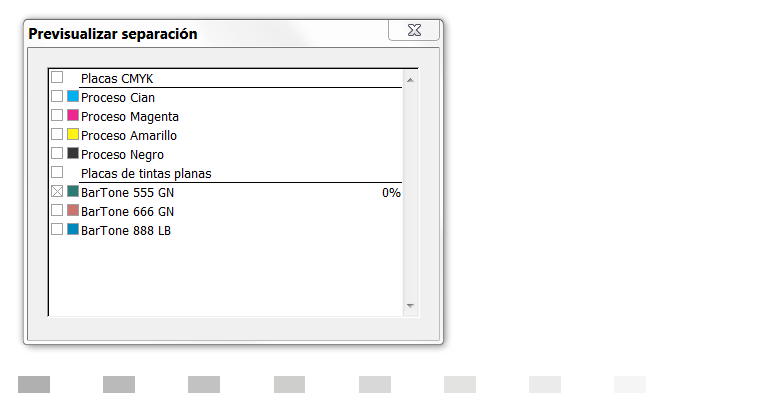
\includegraphics[width=\linewidth]{colorspaceshade.png}}
\caption{Plate for the \texttt{foo} spot color as shown by Adobe
Acrobat. Note both \texttt{foob} and \texttt{foolab},
defined in this document, are listed, too.}
\end{figure}

\section{Page color spaces}

Each PDF page must know which colors will be used (other than the
predefined CMYK, RGB and Gray). By default, \textsf{colorspace} turns
on for every page all newly defined colors, and that will be fine in
most cases. However, you may want to set explicitly the list (for
covers or plates). Use this feature with care, because (1) the
asynchronous nature of \TeX{} (remember it affects the whole current
page), and (2) each distinct color list creates a PDF resource.

\begin{decl}
|\pagecolorspace{<color-list>}|\\
|\resetpagecolorspace|
\end{decl}

To change the color space for a page and the subsequent ones, you can
set something like:
\begin{verbatim}
\pagecolorspace{name1,name2,name3}
\end{verbatim}
(It can be empty.) To return to the default color space, which
contains all the defined spot colors, use \verb|\resetpagecolorspace|.

\section{ICC based spaces}

\begin{decl}
  |\definecolorspace*{<latex-name>}{iccbased}{<icc-file>}|
\end{decl}
The starred version \verb|\definecolorspace*| does not define a new
color model, but sets the behaviour of the three basic color spaces
(CMYK, RGB and Gray).  When belonging to the same space, the last
definition for that space takes precedence and it is considered the
default one. It cannot be used to define new colors or set
them. Currently, only a type is supported -- \verb|iccbased|.  For
example,
\begin{verbatim}
\definecolorspace*{sRGB}{iccbased}{sRGB Profile.icc}
\end{verbatim}

The space it applies to is read from the ICC profile.

The name can be used in \verb|\pagecolorspace|. Alternatively, there
are 3 reserved names: \verb|*rgb|, \verb|*gray|, \verb|*cmyk|, which
stand for the last-defined, default ICC based spaces. Named ICC based
spaces are not set by \verb|\resetpagecolorspace|, but the starred
named are. On the other hand, the starred names are not set
automatically by |\pagecolorspace|, and you must set them explicitly
if you want them to be active.

\begin{note}
  Those ICC spaces do not go to the output intent dictionary (see
  the \textsf{pdfx} package). The latter, as the PDF reference
  explains, supplements rather than replaces the ICC profiles in a
  default color space.
\end{note}

\begin{example}
  Given the following declarations:
\begin{verbatim}
\definecolorspace*{sRGB}{iccbased}{sRGB Profile.icc}
\definecolorspace*{colormatch}{ColorMatchRGB.icc}
\end{verbatim}
  and remembering the RGB space is always active (like the CMYK and
  Gray ones),
\begin{verbatim}
\pagecolorspace{}
\end{verbatim}
leaves the RGB space unprofiled;
\begin{verbatim}
\pagecolorspace{sRGB}
\end{verbatim}
sets the RGB space to sRGB; while the following are (in this
particular example) equivalent:
\begin{verbatim}
\pagecolorspace{colormatch}
\pagecolorspace{*rgb}
\resetpagecolorspace
\end{verbatim}


\end{example}

\section{Overprinting}

This is usually a pre-print task, but by setting it in the document
you will get a better idea of how the colors are actually overlapped
in soft proofing. However, remember the effect produced is
device-dependent, and colorant overprint decisions should be made at
output time (according to the PDF reference).

Very often, it is set for the whole document with the package options
\verb|knockout| (no overprint), and \verb|overprint|. By default, the
overprint mode is 1, but it can be changed with \verb|opm=0|.

Once set the overprint state for the whole document, you can use
something like:
\begin{verbatim}
{\overprintstate{1}text}
\textoverprint[1]{text}
\end{verbatim}
(or \verb|0|, or \verb|no|; default in \verb|\textoverprint| is
\verb|1|, except with the package option \verb|opm=0|).

Since the color stack is used, pdf\TeX{} $\ge$ 1.40 is required.

\begin{warning}
  Some PDF viewers ignore this setting.
\end{warning}

\section{Version}

1.1.1. No new features. Just internal changes related to
\textsc{luatex} and new manual.

1.2.0. CIE LAB spot colors and |illuminant|. Manual rewritten.

\end{document}







